\chapter{Az ókori Egyiptom művészete} % Introduction
\label{ch:1_okri_egyiptom}

\section{Az ókori egyiptom társadalmi felépítése, hiedelemvilága, művészeti korszakai és emlékei}

\vspace{0.5cm}

\tcbox[left=0mm,right=0mm,top=0mm,bottom=0mm,boxsep=0mm,
toptitle=0.5mm,bottomtitle=0.5mm,title=\centering{A tétel adatai}]{%
	
	\begin{tabular}{| p{0.25\textwidth} | p{0.75\textwidth} |}
		
		\centering{\textbf{Tétel teljes címe}}
		&
		Mutassa be az ókori Egyiptom társadalmi felépítését, hiedelemvilágát! Ismertese az ókori egyiptomi művészet korszakait, az építészet, szobrászat és festészet ránk maradt emlékeinek jellegzetességeit!
		\\\hline
		
		\centering{\textbf{Jegyzetek}}
		&
		\begin{compactitem}
			\item Az ókori egyiptomi művészet korszakai, földrajzi, társadalmi környezete.
			\item A sír- és templomépítészet típusai, felépítése, jellmzői.
			\item A szobrászat, a festészet és tárgykultúra jellemzői és stílusjegyei.
		\end{compactitem}
\end{tabular}}\hfill

\subsection*{Földrajzi elhelyezkedés}

\begin{figure}[H]
	\centering
	\tcbox[colback=gray!85!black,
	left=0mm,right=0mm,top=0mm,bottom=0mm,boxsep=1mm,toptitle=0.5mm,bottomtitle=0.5mm,
	title=\centering{Az ókori Egyiptom a Nílus mentén feküdt}]{
		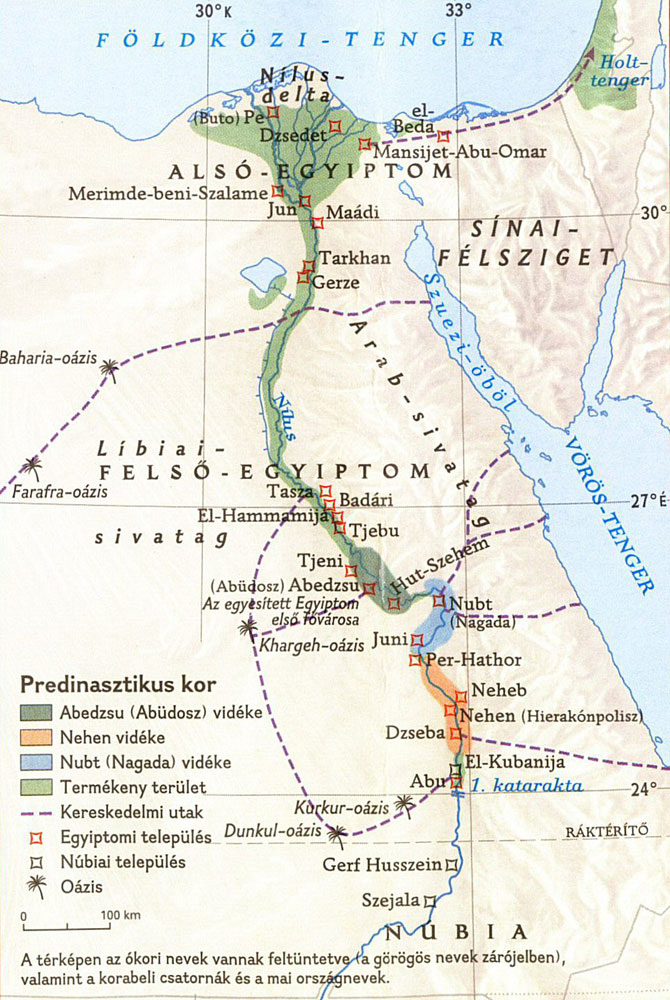
\includegraphics[width=0.9\linewidth]{images/01/egyiptom_terkep}}
	\captionsetup{labelformat=empty}
	\caption{}
\end{figure}

Egyiptom éghaljata alapvetően sivatagos, ezért a kultúra a \textbf{Nílus mentén}, annak partján 5-10 km-es szélességben, több mint 1 000 km hosszan alakult ki.

Ezen ókori civilizáció kialakulásának feltétele a folyó éltető ereje volt: a Nílus. A folyó vetés előtt, júliustól novemberig áradt, termékeny iszapot terítve szét, tápanyagban gazdaggá téve a talajt és lehetővé tette az \textbf{elárasztásos gazdálkodás}t.

A terület földrajzilag és kezdetben politikailag is két részre tagolódott. \textbf{Alsó Egyiptom} északon, a Nílus deltatorkolatánál feküdt a sík vidéken. \textbf{Felső Egyiptom} attól délebbre, a magasabban fekvő területeken, a Nílus mentén hosszan kanyargó partszakaszon helyezkedett el.

\subsection*{Társadalmi felépítés}

\begin{tcolorbox}[enhanced,colframe=gray!50!white,
	colbacktitle=gray!15!white,
	coltitle=gray!50!black,
	borderline={0.5mm}{0mm}{gray!15!white},
	borderline={0.5mm}{0mm}{gray!50!white,dashed},
	attach boxed title to top center={yshift=-2mm},
	boxed title style={boxrule=0.4pt},
	title=Az ókori Egyiptom társadalmi felépítése]{
			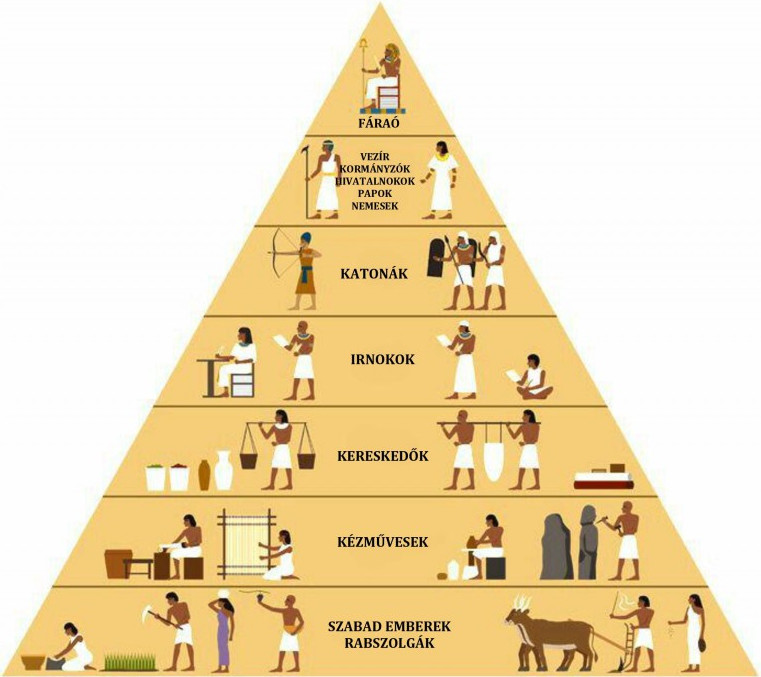
\includegraphics[width=1.0\linewidth]{images/01/egyiptomi_tarsadalom}}
\end{tcolorbox}

Az állam élén a korlátlan hatalommal rendelkező \textbf{fáraó} állt. Az előkelőket a származás szerinti arisztokrácia alkotta, belőlük kerültek ki a főtisztviselők. Az államigazgatás és az igazságszolgáltatás vezetője a vezér. A gazdasági élet irányítószerve a kincstár, az államgépezet működését az írnokok biztosították.

A közigazgatási egységek a nomoszok (kerületek), élükön a nomarkhoszokkal (kormányzókkal). A közrendűeket két réteg alkotta: a parasztok - a föld használata fejében terménnyel és közmunkával adóztak -, és a kézművesek. A házi rabszolgák a hadifoglyokból kerültek ki.\\

\begin{compactitem}
	
	\item\textbf{ Fáraó}: a trón betöltése általában a primogenitura elve (elsőszülött öröklése) történik.\\
	\textit{A fáraó volt a hadsereg főparancsnoka, az államigazgatás és a kincstár feje, valamenynyi templom főpapja és a legfőbb bíró. Mindezeken túl úgy gondolták, hogy rajta múlik az ország termékenysége. Ő tette a földeken az első kapavágást, és ő kezdte meg az aratást.}
	
	\item\textbf{ Papi arisztokrácia}\\
	\textit{A papok - egyiptomi felfogás szerint - csupán az uralkodót helyettesítették kultikus funkcióiban. Hisz a legfőbb pap a fáraó volt! Az egyiptomi papság két fontos funkciót látott el: az istenek kultuszának szolgálatát a templomokban és a halottakról való gondoskodást, az áldozatok bemutatását.}
	
	\item \textbf{Katonai arisztokrácia}\\
	\textit{A fáraó hatalmának alapja a felügyelete alatt álló oikosz-gazdaság és a zsoldos hadsereg volt mely akatonai arisztokrácia megszilárdulásával vált lehetővé. A katonai tisztségviselők elsősorban a társadalom tehetősebb képviselői voltak: előkelők, nagyobb földbirtokosok.}
	
	\item \textbf{ Írnokok} (tisztviselők) (nyilvántartás, adóztatás)\\
	\textit{Az egyiptomi állam legfontosabb hivatalnoka volt. Az irnokok készítették a legfontosabb feljegyzéseket, összeírásokat, a különböző vallási, orvosi, irodalmi szövegeket. Az írástudás minden hivatal elnyerésének feltétele volt. Egy-egy előkelő tucatnyi irnokot foglalkoztatott, s az írnokból akár magas méltóság is válhatott.}
	
	\item \textbf{Kézművesek}\\
	\textit{A Der-el-Medinában élő, kézműves férfiaknak és nőknek tíz napos időszakokra el kellett hagyniuk a várost és családjukat, hogy dolgozni menjenek oda, ahová a fáraó és legfőbb tanácsadói parancsolták. Rövid pihenési időszak után a munkások újabb tíz napot dolgoztak.}
	
	\item\textbf{ Közrendű szabadok}\\
	\textit{A közrendű szabadok foglalkozás szerint földművesek, kézművesek és kereskedők lehettek. A "félszabadok" az ún. királyi munkások, a földbirtokhoz kötött - főleg - parasztok.
	Fontos tény továbbá, hogy a piramisokat nem rabszolgák építették, hanem a közrendű, szabad népesség.}

	\item \textbf{Parasztok}: középítkezések az áradások idején
	
	\item \textbf{Rabszolgák}\\
	\textit{A rabszolgák döntően hadjáratok folyamán kerültek Egyiptomba. Már az i.e. 2700 kö-rül keletkezett „ palermói kő „ is beszámolt arról, hogy egy núbiai hadjárat  után 7000 foglyot hurcoltak az országba.}
\end{compactitem}

\vspace{0.5cm}

Az ókori egyiptomiak úgy hitték, hogy hajdanában nem voltak földi királyok, hanem maguk az istenek uralkodtak az ország felett. Ozirisz volt az, aki földművelésre tanította az embereket. Az ő felesége volt Ízisz, fiuk pedig Hórusz, a sólyomisten. A hór szó valójában magasröptűt, magasságot is jelentett, ezért származtatták magukat tőle az uralkodók. \textbf{Az egyiptomiak királyaikat tehát az istenek földi képviselőjének tekintették.}

\subsection*{Írásmód}

	\begin{wrapfigure}{r}{0.23\textwidth}
		\tcbox[colback=darkgray!85!black,
		left=0mm,right=0mm,top=0mm,bottom=0mm,boxsep=1mm,toptitle=0.5mm,bottomtitle=0.5mm,
		title=\centering{A rosettei kő}]{
		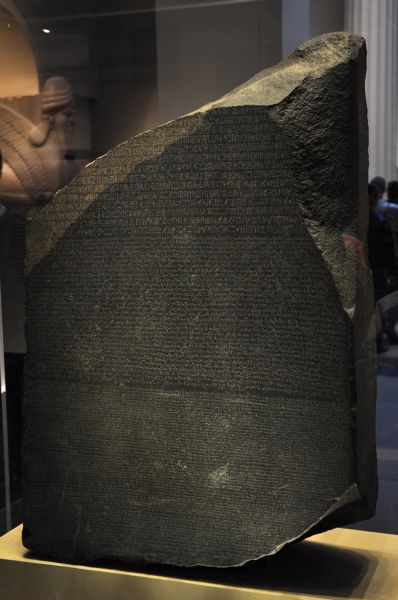
\includegraphics[width=1.0\linewidth]{01/rosetti_ko}
	}
	\end{wrapfigure}

	A legismertebb írásmód a \textbf{hieroglifa} (a szó görög eredetű és „szent vésetet” jelent), \textbf{elsősorban a falakra került és a kultuszhoz} [= a vallásgyakorlat, a vallásos szertartások összessége] \textbf{kapcsolódott}.
	
	Maguk az egyiptomiak írásukat a \textit{medu netjeru}, „az istenek szavai” névvel illették, ezzel is utalva a legendára, mely feltalálását Thot istennek tulajdonítja.
	A hieroglifa-írást 1822-ben fejtette meg Francois Champollion [sampolion] francia tudós, az ún. rosette-i kő alapján, amely egy olyan kőtábla volt, amin ugyanaz a szöveg három nyelven volt olvasható többek közt görög betűkkel.
	
	\begin{tcolorbox}[enhanced,colframe=gray!50!white,
		colbacktitle=gray!15!white,
		coltitle=gray!50!black,
		borderline={0.5mm}{0mm}{gray!15!white},
		borderline={0.5mm}{0mm}{gray!50!white,dashed},
		attach boxed title to top center={yshift=-2mm},
		boxed title style={boxrule=0.4pt},
		title=A hieroglif írás]{
			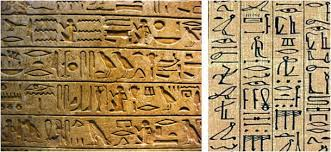
\includegraphics[width=1.0\linewidth]{images/01/hieroglifa}}
	\end{tcolorbox}

	Az írás leggyakoribb alapanyaga - a sírfalakon kívül - a papirusztekercs volt. A háromszög keresztmetszetű papirusznád belső rostjait kivették, hosszú csíkokra vágták, 6 napig vízbe áztatták, függőlegesen majd ezekre keresztbe egymásra helyezték a csíkokat (tulajdonképpen egy fonatot hoztak létre). Majd újabb 6 napon keresztül összepréselték, kiszárították, végül a lapokat a végüknél egymáshoz ragasztották, így jött létre az összegöngyölhető tekercsforma a könnyebb tárolhatóság érdekében.
	

\subsection*{Hiedelemvilág}

Az egyiptomiak egyes természeti jelenségekben természetfölötti erőknek a megtestesülését látták, melyet a hieroglif írásban, a művészi ábrázolásokban emberi, állati, növényi vagy akár egy tárgy alakjában mintáztak meg. 

Egy-egy isten megjelenhetett nemcsak emberi, hanem állati alakban is, sőt nagyon gyakran az emberi testet állatfejjel olvasztották egybe. Ugyancsak lényeges volt az istenek elnevezése is, ami jellemezte viselőjét: az Elrejtett, az Alkotó, a Hatalmas, stb. A vallásos hiedelmek között nagy szerepe volt a mágiának, hisz az egyiptomiak felfogása szerint egy természetfeletti erő igénybe vétele kellett mindenféle baj, veszedelem, betegség leküzdéséhez. Ilyen természetfeletti erőt tulajdonítottak a különböző varázsszövegeknek.

Elképzelésük szerint a fáraó, akit Hórusz földi helytartójának tartottak szintén varázserőt sugárzott. A fáraónak a napisten, Ré fiaként való tisztelete az Óbirodalom közepétől vált általánossá.

Az isteni erők sokféleképpen való megtestesítése mellett az egyiptomi vallás egyik legjellemzőbb részei a \textbf{napkultusz} és a \textbf{halottkultusz}. Ahogy a földi élet \textbf{Ré} (napisten) napsugarainak eredménye, úgy a halál utáni továbbélés, a fennmaradás lehetőségét az Ozirisz-hit adta, s ennek része volt a mumifikálás, amivel a halott túlvilági életét akarták biztosítani.

Az egyiptomi vallás egészén két tényező hatása vonul át: a szellemhité, mely mint lélekhit az egyiptomiak páratlanul fejlett halott- és őskultuszát táplálja; továbbá a vele párosult varázslaté, mely áthat a vallásra, átalakítja az istenek erejéről való felfogást, az isteneket aláveti a varázsszövegeknek, a halottakat mentesíti az erkölcsi felelősség alól az ítéleten, alapjává lesz a király és az egyedek istenné válásának.

A vallás gyakorlásának helyei a templomok voltak, melyek egyben iskoláikkal, könyvtáraikkal a tudománynak, a művelődésnek és a teológiai irodalomnak is a centrumaiként szolgáltak.

\subsubsection*{Többistenhit, fontosabb istenek}

\begin{compactitem}
	\item \textbf{Ré} (vagy Rá, kérdéses): napisten, az emberiség atyja.
	\item \textbf{Hórusz}: az istenek királya a Földön. A mitológiában Ozirisz és Ízisz fia, és az ég ura.
	\item \textbf{Ízisz}: anyaistennő, az Ókori Egyiptom egyik leghíresebb istennője, a varázslás, a termékenység, a víz és szél, a tengerhajózás istennője, a nőiesség és a hűség szimbóluma, Ozirisz felesége, Hórusz anyja.
	\item \textbf{Ozirisz}: a túlvilág birodalmának királya és bírája. Az egyik főisten. Ízisszel és Hórusszal alkot istenháromságot. A túlvilág és a halottak istene, az alvilág életet adó ura, a termőföld istene, ő tanította meg az embert a földművelésre.
	\item Anubisz: az alvilág és holtak oltalmazója, és a bebalzsamozás istene. Fekvő sakál- vagy vadkutyaként ábrázolták, illetve sakál- vagy kutyafejű emberként. Anubisz bíraként van jelen a szív megmérésénél, amikor is a halott szívét egy mérlegre teszik, a másik serpenyőbe pedig Maat-nak, az igazság istenének tollát rakják. Ha a szív nehezebb, akkor azt felfalja Ammut, egy alvilági szörny. Ő tartja számon a holtak szívét.
	\item Széth: a vihar és káosz istene.
	\item Thot (vagy Dzsehuti): a bölcsesség és a Hold istene. Íbiszként vagy kutyafejű páviánként ábrázolták. A civilizációt hozta el az embereknek.
	\item Szobek: az istenek őrzője, krokodilisten.
	\item Hathor, az Égi Tehén: Azonosult Básztettel, a termékenység és a szerelem istennője, tehén képében jelenik meg, Íziszhez hasonlították, bár a két istennő egymástől teljesen különbözött.
	\item Ámon: az istenek királya, ugyanaz mint Ámon-Ré, a napisten.
\end{compactitem}

\vspace{0.5cm}

\begin{tcolorbox}[enhanced,colframe=gray!50!white,
	colbacktitle=gray!15!white,
	coltitle=gray!50!black,
	borderline={0.5mm}{0mm}{gray!15!white},
	borderline={0.5mm}{0mm}{gray!50!white,dashed},
	attach boxed title to top center={yshift=-2mm},
	boxed title style={boxrule=0.4pt},
	title=Az ókori Egyiptom istenei]{
		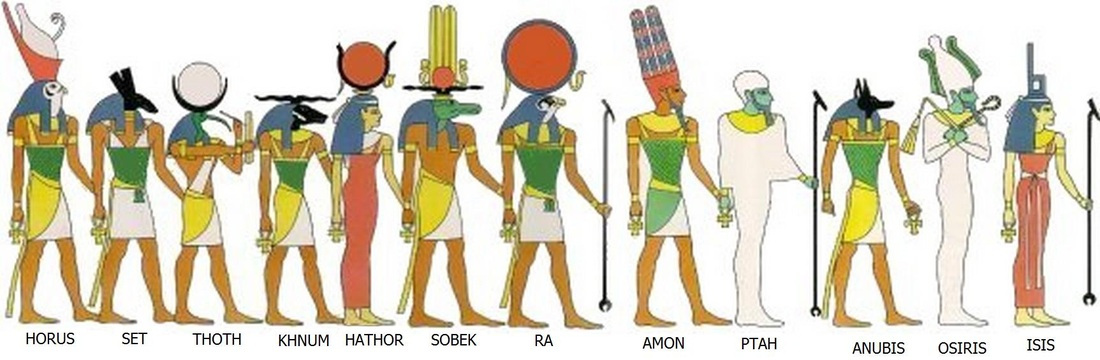
\includegraphics[width=1.0\linewidth]{images/01/istenek}}
\end{tcolorbox}

\subsection*{Halottkultusz, temetkezési szokások}

	Az egyiptomi hitvilág szerint \textbf{az embernek két lelke volt}:\textbf{ az egyik a Ba nevű test-lélek} (tulajdonképpen maga a test), \textbf{a másik a Ka nevű szellemi lélek} (életadó energia, a test állandó tanácsadója, lelkiismerete [ma talán pszichének neveznénk]). A szellemi lélek a vélekedés szerint azonban csak addig él, amíg a testlélek is, ezért a testet meg kellett őrizni az örökkévalóságig, a szellemi lelket pedig táplálni kellett. (A test megőrzését szolgálta a mumifikálás és a masszív sírépületek, a piramisok.) A hitvilág szerint a szellemi lélek minden éjszaka lemegy az alvilágba, majd minden reggel a nappal együtt újjáéled. Az élet tehát mindig Kelethez, a napkeltéhez, a halál mindig Nyugathoz, a naplementéhez kapcsolódott, ezért temetkeztek az egyiptomiak minden korszakban a Nílus bal, azaz nyugati partjára.
	
	\textbf{A test megőrzésének módja a mumifikálás volt.} (Az eljárás kiindulása bizonyára az volt, hogy a predinasztikus korban a száraz sivatagi homokba temetkeztek, ami kiszívta a test nedvességét, ezáltal meggátolta a hús bomlását.) A műveletet papok végezték a sírok mellett lévő halotti templomban:
	\begin{compactitem}
		\item Az elhunyt belső szerveit kivették, kiszárították és az ún. kanopusz-edényekbe helyezték.
		\item Az agyat az orron keresztül eltávolították, a testet és a koponyát gyantával, szurokkal töltötték ki.
		\item A testet tartósító sós lébe áztatták, 70 napig a napon szárították, bebalzsamozták, végül vászonszalagokkal légmentesen bepólyálták.
	\end{compactitem}

\begin{figure}[!h]
	\begin{minipage}{0.49\textwidth}
		\centering
		\tcbox[colback=darkgray!85!black,
		left=0mm,right=0mm,top=0mm,bottom=0mm,boxsep=1mm,toptitle=0.5mm,bottomtitle=0.5mm,
		title=\centering{Kanópuszedények}]{
			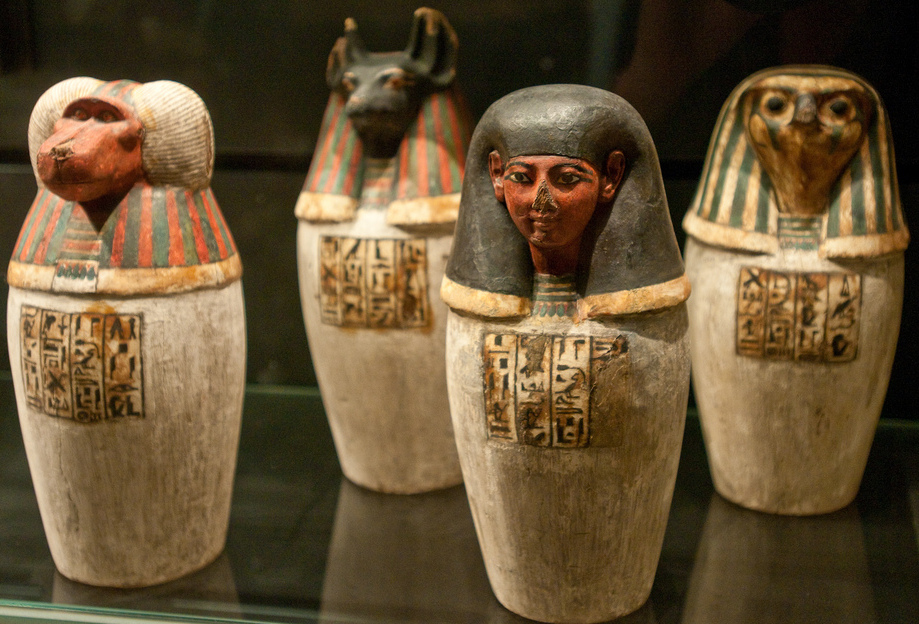
\includegraphics[width=1.0\linewidth]{01/kanopusz}
		}
	\end{minipage}\hfill
	\begin{minipage}{0.45\textwidth}
		\centering
		\tcbox[colback=darkgray!85!black,
		left=0mm,right=0mm,top=0mm,bottom=0mm,boxsep=1mm,toptitle=0.5mm,bottomtitle=0.5mm,
		title=\centering{Múmia ábrázolása}]{
			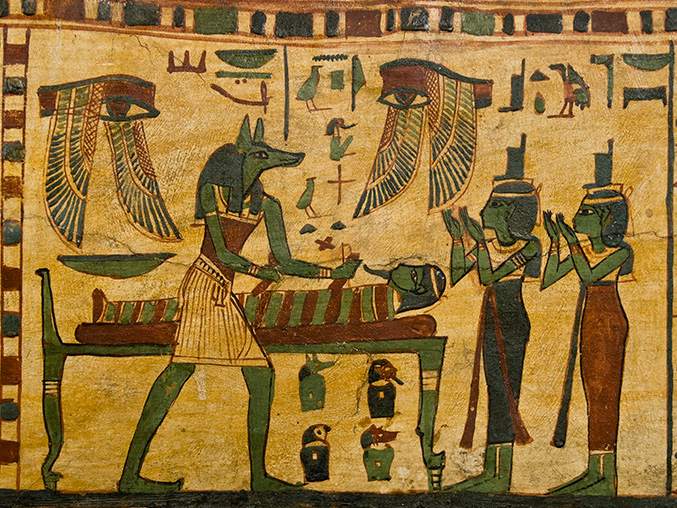
\includegraphics[width=1.0\linewidth]{01/mumia}
		}
	\end{minipage}\hfill
	\captionsetup{labelformat=empty}
	\caption{}
\end{figure}

	

\subsection*{Művészeti és birodalmi korszakok}

	Az egyiptomi művészet nem díszítésre szolgáló vagy történeteket elmesélő művészet volt, hanem kifejezetten gyakorlati funkciót töltött be: a halottkultusz része volt. Az építészetben megjelenő formáknak, a sírfestészet, sírszobrászat témáinak és stílusának mind az egyiptomi hitvilágban, mitológiában találhatjuk meg a magyarázatát.

Egyiptom történelmének nagy részét három „birodalmi” szakaszra lehet osztani (melyek a művészet szempontjából is meghatározóak voltak): az óbirodalmi szakaszra, a középbirodalmi szakaszra és az újbirodalmi szakaszra. Ezeket rövidebb átmeneti időszakok választották el egymástól. Az „átmeneti” szó itt arra utal, hogy ezekben az időkben Egyiptom nem állt egységes politikai uralom alatt, hanem más, erősebb birodalmak uralma alá került. Az egyiptomi civilizáció alapjait jóval az Óbirodalom kora előtt a Nílus folyó partján letelepülő emberek által létrehozott öntözéses földművelés fektette le, amely a városok és specializált gazdasági tevékenységek (például a kézművesség, bányászat) kialakulásához vezetett.

\tcbox[left=0mm,right=0mm,top=0mm,bottom=0mm,boxsep=0mm,
toptitle=0.5mm,bottomtitle=0.5mm,title=\centering{Az ókori Egyiptom korszakai}]{%
	
	\begin{tabular}{| p{0.21\textwidth}|p{0.15\textwidth} | p{0.55\textwidth} |}
		
		\centering{\textbf{Óbirodalom}}
		&
		kb. Kr. e. 2600-2100
		&
		Híres fáraók: Dzsószer, Kheopsz, Kefrén, Mükerinosz.
		\\\hline
		
		\centering{\textbf{Középbirodalom}}
		&
		?
		&
		???
		\\\hline
		
		\centering{\textbf{Újbirodalom}}
		&
		?
		&
		???
		\\\hline
		
		\centering{\textbf{Kései kor}}
		&
		?
		&
		???
		\\\hline
\end{tabular}}\hfill

\subsection*{Az Óbirodalom művészete (kb. Kr.e. 2600-2100)}

Első fáraója Dzsószer volt, majd utána a leghíresebb egyiptomi uralkodók következtek: Kheopsz, majd az ő fia, Kefrén, és unokája Mükerinosz. Az országot ekkor 42 kerületre osztották, melyek élén egy-egy ún. vezír, azaz hivatalnok állt. Ennek az időszaknak a legfontosabb emlékei az említett négy fáraó piramisai Szakkarában és Gízában, a fáraók piramisai és szobrai.

\subsubsection*{Piramis-építészet}

\paragraph{Funkció} A piramisok az egyiptomi uralkodók sír-építményei voltak. Céljuk a halott fáraó mumifikált testének megőrzése volt, valamint hatalmas méreteikkel a fáraó nagyságát szimbolizálták. A piramisok tetején egy aranyból készült piramidion volt: a piramist felül lezáró kissebb piramis (15-20 méter magas). Mivel a nap fényét visszaverte, csillogásával mindenfelé jelezte a hatalmas fáraó sírjának helyét. (Ezek már nincsenek meg.)

\paragraph{Építőanyag} A piramisokat mészkőtömbökből építették, amit helyben bányásztak, és szabályos téglatest formájúra faragtak. A tömbök között semmilyen kötőanyagot nem használtak. A nagyméretű kőtömböket úgy szállították, hogy a sivatagi homokon egy iszap-utat hoztak létre, amin a kőtömb könnyedén csúsztatható volt, mindössze 6 emberre volt szükség így a szállításához. Néhány esetben - a belső kamrákban - gránitot is használtak, ami a legnehezebb és a legkeményebb kőfajta. A kemény kövek használata is kifejezi, hogy a piramisokat az örökkévalóság számára építették.

\paragraph{Építők} A piramisokat építő rabszolgákról Hérodotosz görög történetíró számolt be, ez a nézet azonban mára elavulttá vált: a helyben élő szabad, fölművelő köznép élelem fejében dolgozott a fáraónak azalatt, amíg a Nílus kiáradt. 

A Gízai piramisok mellett megtalálták a munkások városát, ami kórháztól kezdve sörfőzdén át mindennel el volt látva, ami csak a mindennapi élethez szükséges. 

Az piramis belül tömör, mindössze néhány sírkamrát és az azokhoz vezető keskeny (1m magas és széles) és meredek folyosókat, valamint szellőző folyosókat tartalmaz. Az építkezés alatt a belső termekbe kívülről tükrök segítségével vezették be a fényt. A piramisok belseje mára szinte teljesen lepusztult, festésnek, díszítésnek nyoma alig maradt. Eredetileg azonban domborművek díszítették a sírkamrák falait.

\paragraph{Sírrablók} A piramisokba a fáraó holteste mellé annak minden tárgyát és számtalan adományt helyeztek, amiket már a legkorábbi időktől kezdve fosztogattak. A kincsek védelmezésére, a sírrablók megtévesztésére a piramis oldalán gyakran egy álbejáratot nyitottak, a valódi bejáratot pedig elfedték.

\subsubsection*{A piramis formájának kialakulása}

\begin{wrapfigure}{r}{0.25\textwidth}
	\tcbox[colback=darkgray!85!black,
	left=0mm,right=0mm,top=0mm,bottom=0mm,boxsep=1mm,toptitle=0.5mm,bottomtitle=0.5mm,
	title=\centering{Masztaba}]{
		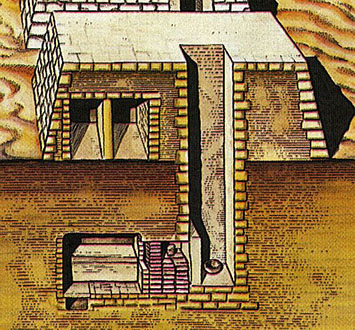
\includegraphics[width=1.0\linewidth]{01/masztaba}
	}
\end{wrapfigure}

\paragraph{1. Masztabák} 
A korai időszakban az uralkodók ún. masztabákba temetkeztek. Ezek a föld alatt lévő sírkamra fölé kerültek, lapos, négyzet alaprajzú, csonkagúla alakú, gyakran egyetlen kőtömbből álló építmények voltak. Masztabák az Óbirodalom idején is készültek, ekkor azonban már nem az uralkodó, hanem a vezír-réteg, vagy a fáraó-feleségek temetkeztek ilyen sírokba.

\begin{wrapfigure}{r}{0.35\textwidth}
	\tcbox[colback=darkgray!85!black,
	left=0mm,right=0mm,top=0mm,bottom=0mm,boxsep=1mm,toptitle=0.5mm,bottomtitle=0.5mm,
	title=\centering{Dzsószer fáraó lépcsős piramisa Szakkarában}]{
		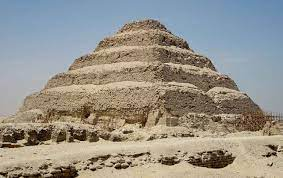
\includegraphics[width=1.0\linewidth]{01/dzsoszer_piramis}
	}
\end{wrapfigure}

\paragraph{2. Lépcsős piramis}
Az Óbirodalom idején az uralkodó megnövekedett tekintélyét, isteni voltát kifejezendő, a lapos masztabák tetejére további szűkebb négyzet-alaprajzú csonkagúlákat helyeztek, hogy magasságát növeljék. Pl.: Dzsószer fáraó lépcsős piramisa Szakkarában.

Dzsószer fáraó piramisa a lépcsős piramisok első példája volt, tulajdonképpen több, egyre kisebb, egymásra rakott masztaba. Szakkarában (a mai Kairótól kb.20 km-re délebbre) található. Kb. 60 m magas, fél-egy méter magasságú mészkőtömbökből épült fel. Alkotója Dzsószer legelső vezírje, papja, orvosa, építésze: Imhotep volt.

\begin{wrapfigure}{r}{0.35\textwidth}
	\tcbox[colback=darkgray!85!black,
	left=0mm,right=0mm,top=0mm,bottom=0mm,boxsep=1mm,toptitle=0.5mm,bottomtitle=0.5mm,
	title=\centering{Sznofru fáraó dahsúri tört falú piramisa}]{
		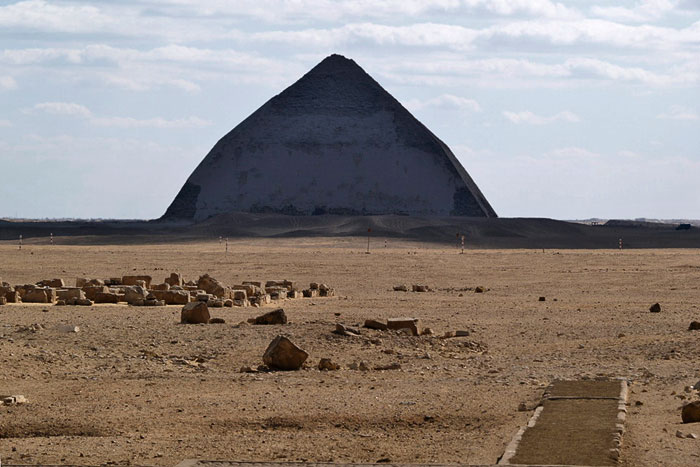
\includegraphics[width=1.0\linewidth]{01/dashur_piramis}
	}
\end{wrapfigure}

\paragraph{3. Tört élű piramis}
Ez az időszak a hatalmas méretű gúla alakzat felépítésének kísérleti szakasza volt. Pl.:t ört élű és tág szögű piramisok Dahsúrban.
A Dzsószer után uralkodó fáraó (Sznefer) már a sok, kis lépcsőfokokból álló gúlaformát próbálta felépíteni. Piramisát azonban homok-alapra építette, és az építkezés közben a kőtömeg alatt megsűllyedt a talaj, a piramis éleinek szögét ezért beljebb kellett dönteni, hogy az építmény alacsonyabb, ezéltal kisebb tömegű legyen. Ennek eredménye lett a dahsúri Tört élű piramis.
A Tört élű piramis közvetlen szomszédságában Sznefer építészei - valószínű, hogy kijavítsák a hibájukat - a Tört élű piramis építésének második szakaszában alkalmazott dőlésszöggel építettek fel egy másik, már valóban a híres gúla-formát mutató sírépítményt, amit a vörös színű mészkövei miatt Vörös piramisnak neveznek.


\paragraph{4. Gúla forma}
\subparagraph{A gúla forma szimbolikája}
A cél elsősorban a magasság növelése volt, hiszen az a fáraó jelentőségét fejezte ki. Másrészt a forma iránti rokonszenv oka az volt, hogy az egyiptomi hitvilágban a gúla-forma több szimbolikus jelentést hordozott. Az egyiptomi teremtés-mítosz ilyennek írta le az ősvízből kiemelkedő őshalmot, azaz az első szárazföldet. A lépcsőzetesség kifejezte a napistenhez, Réhez vezető utat, amin a fáraó szellemi lelke felment az egekbe. A forma hasonló volt a fentről szétágazó nap sugaraihoz, azaz kifejezte Ré, a napisten védelmét az eltemetett fáraó felett. Továbbá minden ősi civilizáció szakrális épülete négyszög alaprajzra kerülő toronyszerű építmény volt - lásd a mezopotámiai zikkuratokat, vagy a maják amerikai templomait, amik hasonló formájúak. A piramis-forma kialakulásának is fontos feltétele volt, hogy ez a forma volt statikailag a legjobban megoldható az ókorban.

\subparagraph{A forma} Az építmény a tökéletességet tükröző szabályos gúla formájú: négyzet alaprajz, amihez minden oldalról a négyzet oldalaival egyenlő hosszúságú oldalú, szabályos háromszögek kapcsolódnak.

\subparagraph{A Gízai piramis-együttes}
Egyiptom legnagyobb piramisát a legidősebb fáraó, Kheopsz építtette (kb.Kr.e.2570-től). Az építkezés több, mint húsz évig tartott, már a fáraó megkoronázásakor elkezdték. A piramis 146m magas (2,3 millió mészkőtömbből építették, amik egyenként másfél méter magas és egy-két méter széles faragott téglatestek, és kb. két és fél tonnát nyomnak).

\begin{wrapfigure}{r}{0.5\textwidth}
	\tcbox[colback=darkgray!85!black,
	left=0mm,right=0mm,top=0mm,bottom=0mm,boxsep=1mm,toptitle=0.5mm,bottomtitle=0.5mm,
	title=\centering{Gízai piramisok}]{
		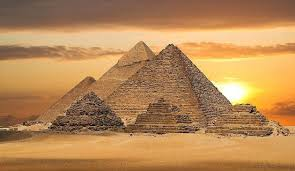
\includegraphics[width=1.0\linewidth]{01/gizai_piramisok}
	}
\end{wrapfigure}

Kheposz piramisa mellett három kisebb piramis is áll, amelyeket felesége és lánytestvérei számára építtetett.
Kheposz fia, Kefrén építette a kissé délebbre álló piramist, ami a fotókon középen áll, és
a három sír-építmény közül a legmagasabbnak tűnik. Ennek csak az az oka, hogy a Kheopsz-piramis szintben lejjebb áll. (Kefrén piramisa 136 m magas.) Az egyetlen, amin fennmaradtak azok a mészkőlapok, amelyekkel
4
ezeket a piramisokat lefedték, hogy a lépcsőzetességet teljesen megszüntetve a sima felületű, (egy hatalmas kristály hatását keltő) szabályos gúlaformát létrehozzák.
A harmadik, még délebbe álló piramis Mükerinosz fáraóé, a legkisebb a trióból, 62m magas.

\subsubsection*{Halotti templomok}

A piramisok mellett halotti templomokat is építettek, ahol a fáraó múmiáját készítették el, illetve a halálával istenné vált fáraónak szentelt templomok szerepét töltötték be az épületek, ahol a fáraó szellemi lelkének áldoztak. Ezek a templomok igen romos állapotban maradtak fenn, a legjobb állapotban megmaradt templom Kefrén fáraóé.

\paragraph{Kefrén halotti temploma Gízában}
A templom Kefrén piramisa előtt áll, mögötte található a Szfinx, így a piramis, a Szfinx és a templom egy tengelyt alkot. A templom hatalmas gránittömbökből épült. Fő részét az a folyosó jelenti, amin a fáraó múmiáját szállították végig. A folyosó két oldalán az istenek szobrai álltak, amiket az ablakokon beeső fény világított meg.

\subsubsection*{Fáraó szobrok}

A fáraó a politika és a vallás feje volt egy személyben. A fáraó szó arab, eredetileg a memphiszi palotát és a palotaőrséget jelentette. A fáraó neve általában egy olyan rövid mondat, ami isteni eredetére utal, pl. „Ré isten fia”

\paragraph{A fáraó uralkodói jelvényei}

	\begin{compactitem}
		\item \underline{Kettős korona:}\\
		Alsó és Felső Egyiptom feletti hatalom szimbóluma. Felső Egyiptomé a fehér - valószínű, hogy ezüstből készült - korona, ami egy csúcsos hegyes sisak volt. Alsó Egyiptomé a piros korona hátul hosszú nyúlvánnyal, elől fémszállal, a homlokán a két terület istenségeinek szimbólumaival, a kobrával és a keselyűvel.
		
		\item \underline{Menész:} a nehéz kettős koronát helyettesítő vászonkendő.
		
		\item \underline{Álszakáll:} bölcsesség, a bölcs uralkodó jelképe.
		
		\item \underline{Pásztorbot alakú jogar:} a népét védelmező uralkodó.
		
		\item \underline{Légycsapó vagy ostor:} az ellenségeit kíméletlenül leigázó uralkodó.
		
		\item \underline{Állatfarok:} a köténye felső részéről lógott le, a harci ügyességekben járatos uralkodó szimbóluma.
	\end{compactitem}

\begin{figure}[H]
	\centering
	\begin{minipage}{0.45\textwidth}
		\begin{tcolorbox}[enhanced,colframe=gray!50!white,
			colbacktitle=gray!15!white,
			coltitle=gray!50!black,
			borderline={0.5mm}{0mm}{gray!15!white},
			borderline={0.5mm}{0mm}{gray!50!white,dashed},
			attach boxed title to top center={yshift=-2mm},
			boxed title style={boxrule=0.4pt},
			title=Kettős korona]{
				
\includegraphics[width=1.0\linewidth]{images/01/kettos_korona}}
		\end{tcolorbox}
	\end{minipage}
	\hfill
	\begin{minipage}{0.45\textwidth}
		\begin{tcolorbox}[enhanced,colframe=gray!50!white,
			colbacktitle=gray!15!white,
			coltitle=gray!50!black,
			borderline={0.5mm}{0mm}{gray!15!white},
			borderline={0.5mm}{0mm}{gray!50!white,dashed},
			attach boxed title to top center={yshift=-2mm},
			boxed title style={boxrule=0.4pt},
			title=Pásztorbot és korbács]{
				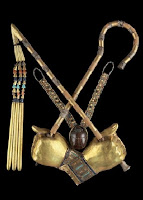
\includegraphics[width=1.0\linewidth]{images/01/pasztorbot_korbacs}}
		\end{tcolorbox}
	\end{minipage}
	\captionsetup{labelformat=empty}
	\caption{}
\end{figure}

\paragraph{A fáraó szobrok rendeltetése}
A fáraók szobrai nem a piramisokban álltak, hanem általában a piramisok mellett lévő halotti templomokban kaptak helyet fülkékben. Nem körüljárhatók, a hátuk gyakran egy laphoz támaszkodik, a figurák szigorúan főnézetre komponáltak.

\begin{wrapfigure}{r}{0.5\textwidth}
	\begin{tcolorbox}[enhanced,colframe=gray!50!white,
		colbacktitle=gray!15!white,
		coltitle=gray!50!black,
		borderline={0.5mm}{0mm}{gray!15!white},
		borderline={0.5mm}{0mm}{gray!50!white,dashed},
		attach boxed title to top center={yshift=-2mm},
		boxed title style={boxrule=0.4pt},
		title=Kefrén fáraó szobra]{
			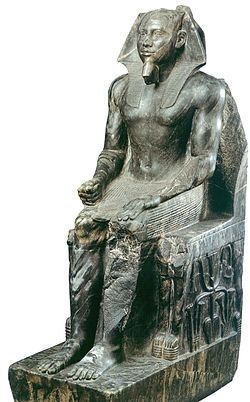
\includegraphics[width=1.0\linewidth]{images/01/kefren_szobra}}
	\end{tcolorbox}
\end{wrapfigure} 

A fáraó-szobor a fáraó halála után egykori ideális testének helyettesítője volt, a visszatérő szellemi lélek számára készítették. Ez volt a jelzés, hogy a lélek tudja, hogy kinek a teste van a templom melletti piramisban. A szobron található ún. kartus - a fáraó nevét tartalmazó ovális alakú jelzés - tájékoztatott a szobor kilétéről. Mivel a visszatérés idejét nem lehetett tudni, a szobornak az örökkévalóságig fenn kellett maradnia, ezért tartós, kemény kőből, a legjobb esteben gránitból készítették. (Ezt délről szállították a Nílus deltájához.)

\paragraph{A fáraószobrok stílus-jellemzői}

A szobor egyben kifejezte azt is, hogy a fáraó halálával istenné vált, így a szobor stílusának minden eleme az isteni tökéletességet kívánja tükrözni.

A fáraóról nem portrét készítettek, hanem a fáraót, mint ereje teljében lévő, kiegyensúlyozott, bölcs, fiatal és szép, azaz ideális és isteni uralkodót örökítették meg a szobrok: nyugodt, mozdulatlan testtartás, frontális beállítás (= minden testrésze a nézővel szembe néz: sem a fej, sem a törzs, sem a lábak nem fordulnak el).

Bal lába mindig előrébb helyezett (de nem lép, mozdulatlan). Magyarázatként szolgálhat erre a testtartásra az, hogy a halálakor a fáraó ezzel fejezte ki az istenek előtt az alázatát, bűnösségét: a szívének volt szüksége támasztásra, ezért kerül mindig a bal láb előbbre.

A tömegkezelés zárt, a szobor egésze tömbszerű, a figura szorosan a combjai mellett tartja a kezét. 

Mereven előrenéző, eszményített arc és tekintet, nyugodt, érzelemmentes, ráncmentes, idealizált, fiatal arc, a fejen általában a menész-korona a kobrával és keselyűvel (Alsó- és Felső-Egyiptom isteneinek szimbólumai, itt azt fejezik ki, hogy ők védelmezik az uralkodó hatalmát a két terület felett).

Az izmokat nem túlhangsúlyozó, finoman, visszafogottan izmos, idealizáló mezítelen felsőtest, egyszerű szoknya.

A kezek ökölbe szorulnak, amiben általában a túlvilági élet kulcsa vagy templomi csörgő van. 

A fáraó-szobrok az Óbirodalom idején általában életnagyságúak, a későbbi korokban méreteik a lehetőségekhez mérten megnőnek, a fáraó nagyságát fejezik ki. (Pl. a Memnón kolosszusok 25 m magasak.)
	
\cleardoublepage

\section{Az ókor meghatározó festészeti techinkái: az egyiptomi falkép}

\begin{center}
	\begin{longtable}{ | m{0.25\textwidth} | p{0.75\textwidth} | }
		
		\hline
		\multicolumn{2}{|c|}{\textbf{A tétel adatai}}
		\\ \hline
		
		\hline
		Tétel teljes címe	
		 &
		 Melyek a meghatározó festészeti technikák az ókorban? Fejtse ki, miként alakult egy egyiptomi falkép elkészítésének munkamenete, milyen alapozást, pigmenteket és kötőanyagot használtak?
		\\ \hline
		
	\end{longtable}
\end{center}